\section{Demonstration}\label{sec:demo}

%In this section, we will discuss the details for the demonstration. 

\begin{figure}[t]
\centering
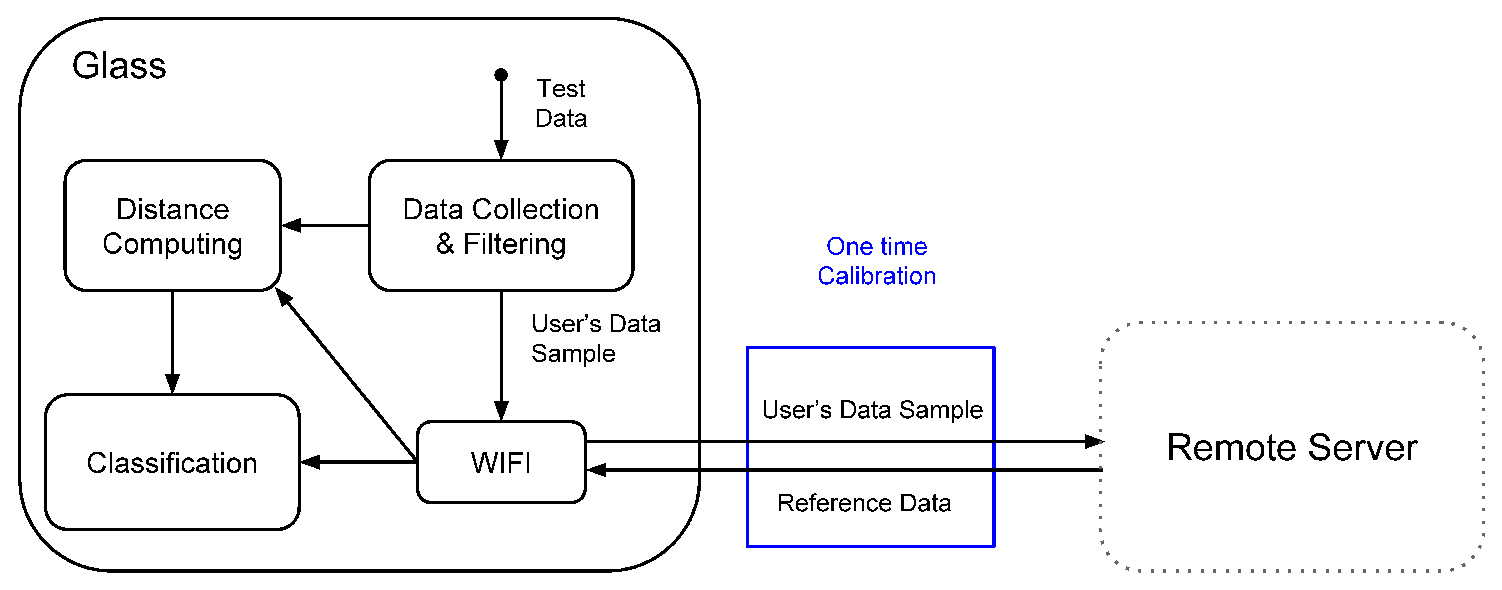
\includegraphics [width=\columnwidth]{pic/software_arch.eps}
\caption{Software modules of \systemname~implementation}
\label{fig:glass-softwarearch}
\end{figure}


\subsection{Headbanger App on GLASS}
We implemented \systemname~ as an app on Google Glass using the Glass Development Kit (GDK)~\cite{gdk}. Fig.~\ref{fig:glass-softwarearch} shows the application components in our implementation. In the initiation phase, the application plays a music cue for a user--specified duration. The user performs head movement by following the music flow while the application is collects accelerometer data. On completion of the music cue, the application enters the processing phase where the sensor data is input to the \systemname~'s software modules for processing. In our current implementation, the computation for the training phase is done on a PC and the template is determined apiori to the online authentication process.
As a result, the app outputs a binary decision which is shown as a textual output on the GLASS's screen; {\em successful} is referred as "Welcome back!", and {\em failed} is referred as "One more try!", as shown in Fig.~\ref{fig:headbanger-illustrate}.


\subsection{Demonstration Setup} 
We will demonstrate \systemname in two authentication modes for login to GLASS : (i) owner authenticating to the device, and (ii) attacker being prevented from login to the device.
For the former, the demo presenter, considered as one of the owners of the GLASS device, will demonstrate a correct authentication movement in order to show the capability of \systemname~to correctly recognize a true user. To demonstrate the robustness of \systemname to attacks, the demo presenter will set up a \lq mimic challenge\rq during the demonstration session.  
The device will be pre--loaded with template samples from 4 voluntary users (each is a potential attacker to others), including the presenter. All of users will have access to viewing a video recording of their head--movement exercise, while they are attempting to use the system, and then given a chance to login to the GLASS. 

At the demo, the attackers will then be allowed to choose one of the users' action to mimic. In this regard, they will be allowed to watch the corresponding video for as long as they feel comfortable to start imitating the system. The demo app will provide a feedback on the similarity of their head--movements to the original, after each attempt, so that the challengers may adjust their actions if necessary. If the attacker fails to login within 10 attempts, the attack is considered to being compromised by our system. Our design uses the fact that, since the music cue is played via a bone--conduction speaker or a earplug, it is difficult to record the music in a normal environment, making it difficult for the attackers to break the system. To ensure fairness during the demo session, we will set the volume on the GLASS to maximum and try to achieve audible quality recording of the music cue played on the GLASS.

During the entire session at the demo, we will screen--cast the Google GLASS's heads--up display screen to an external monitor for audiences and participants to emulate a real--time testing environment of our system.

%\begin{figure}[t!]
%\centering
%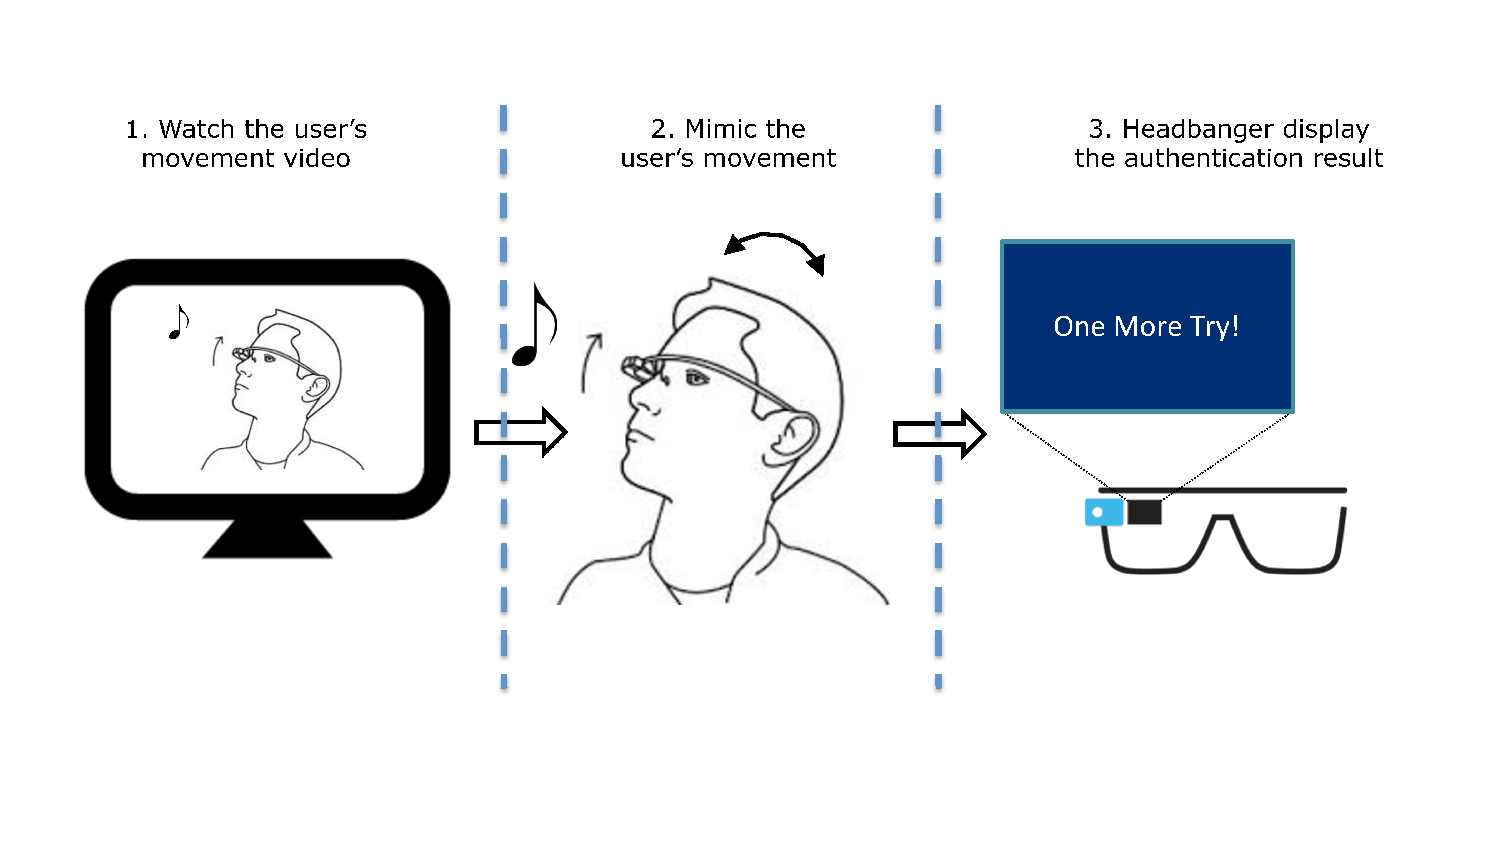
\includegraphics[width=\columnwidth]{pic/demo_illus.eps}
%\caption{Illustration of Headbanger demo. The challenger first watch the video of the user's authentication movement. As long as the challenger feels he can remember the movement, he starts his mimic attacker.Finally, \systemname~displays the authentication result on the screen. }
%\label{fig:headbanger-illustrate}
%\end{figure}